\begin{tikzpicture}[font=\footnotesize]
\node (A) at (0,0) {\Alice};
\node (B) [right of = A, node distance = 4cm] {\Bob};
\node (0a) [below of=A, node distance=1cm] {$N, e, m^e \bmod N$};
\node (0b) [below of=B, node distance=1cm] {};
\draw[-latex] (0a) -- (0b) node [midway,above] {};
\node (1a) [below of=0a, node distance=0.5cm] {};
\node (1b) [below of=0b, node distance=0.5cm] {a random $x$};
%\draw[-latex] (1a) -- (1b) node [midway,above] {};
\node (2a) [below of=1a, node distance=0.5cm] {};
\node (2b) [below of=1b, node distance=0.5cm] {$x^2 \bmod N$};
\draw[-latex] (2b) -- (2a) node [midway,above] {};
\node (3a) [below of=2a, node distance=0.5cm] {the square root $y$ of $x^2$};
\node (3b) [below of=2b, node distance=0.5cm] {};
\draw[-latex] (3a) -- (3b) node [midway,above] {};
\node (4a) [below of=3a, node distance=0.5cm] {};
\node (4b) [below of=3b, node distance=0.5cm] {$y \overset{?}{=} \pm x$};
\end{tikzpicture}
